%======================================================================================================
%======================================================================================================
% PLANTILLA PARA INFORMES T�CNICOS de la DAS de la DIIV
%  Versi�n 1.35 del 27/8/2015
% 	-Rearmado de portada. Mayor sobriedad y destaque del t�tulo del informe t�cnico.
%	-Incorporados fixes varios para poder referir secciones y que no aparezcan '.' al final.
%	-Incorporado par�metro para que no se estire hasta el final los �tems del glosario.
%	-Afectada la geometr�a: tiene menor margen en toda direcci�n.
%	-Cambio de color rojo a negro t�tulos varios.
%	-Modificado apa-good.bst --> italizado el "et al"
%======================================================================================================
%======================================================================================================


% =====================================================================================================
% =====================================================================================================
% PRE�MBULO
% =====================================================================================================
% =====================================================================================================

\documentclass [11pt]{article}
\usepackage[T1]{fontenc} % para que pueda partir palabras con acentos
\usepackage[latin1]{inputenc}
\usepackage{rotating}
\usepackage{graphicx, nicefrac}
%\usepackage{graphicx}
\usepackage[spanish]{babel} % Ojo que esto cambia el nombre de las secciones
\usepackage{times,url}
\usepackage{amsmath}
\usepackage{mathrsfs}
\usepackage{amsfonts}
\usepackage{amssymb}
%\usepackage{hyphen}
\hyphenation{EAMMRA}
\usepackage{fullpage}

\usepackage[ampersand]{easylist}

\usepackage[a4paper,bottom=2.7cm,top=2.7cm,left=2.5cm,right=2.5cm]{geometry}
\usepackage{fancyhdr} % Esto cambiar� la ubicaci�n de los numeritos de las p�ginas
\usepackage{grffile} % Para tipear nombres de archivo con espacios
%\usepackage{esvect} % Para poner flechas de vector m�s copadas
\usepackage{array} % Paquete que mejora la funcionalidad de array

% Estilo de p�gina

\fancypagestyle{plain}{%redefining plain pagestyle
	\fancyhf{} %clear all headers and footers fields
	\fancyfoot[R]{\thepage} %prints the page number on the right side of the header
	\renewcommand{\headrulewidth}{0pt}
	\renewcommand{\footrulewidth}{0pt}
	}
\pagestyle{plain}

% M�s paquetes extra

\usepackage[usenames,dvipsnames]{color}
\usepackage{colortbl}
\usepackage{tocloft}
\usepackage{setspace}
\usepackage{titlesec}
\usepackage{fix-cm}
\usepackage{natbib}
\setcitestyle{square}
\usepackage{multirow}
\usepackage{bigstrut}

\usepackage{wrapfig}
\usepackage{enumitem}
\usepackage{appendix}

\usepackage{listings}
\usepackage{graphicx}
\usepackage{multirow}


\renewcommand{\appendixtocname}{AP�NDICES}
\renewcommand{\appendixpagename}{\Large\bf\textcolor{black}{AP�NDICES}}

% Formateo de los caption de figuras y tablas

\usepackage[margin=10pt,font=small,labelfont=bf,labelsep=period]{caption}
\DeclareCaptionListFormat{formato}{\textcolor{black}{\textbf{{#1 #2}}}}
\captionsetup{listformat=formato,labelfont={bf}}


\renewcommand{\cftfigpresnum}{\textcolor{black}{FIG. }}
\setlength{\cftfignumwidth}{1.5cm}
\renewcommand{\cfttabpresnum}{\textcolor{black}{TABLA }}
\setlength{\cfttabnumwidth}{2.25cm}  

% Formateo general de los t�tulos

%% \def\thesection{\Roman{section}}
%% \def\thesubsection{\thesection .{\arabic{subsection}}}
%% \def\thesubsubsection{\thesubsection .{\alph{subsubsection}}}
%% \def\theappendix{\arabic{appendix*}.}

%=============================================================================

% Nueva definicion de secciones:
\makeatletter
\renewcommand\section{\@startsection{section}{1}{\z@}%
                                   {-2.5ex \@plus -1ex \@minus -.2ex}%
                                   {2.5ex \@plus.2ex}%
                                   {\normalfont\large\bfseries\color{black}}}
\renewcommand{\thesection}{\Roman{section}}
\renewcommand{\@seccntformat}[1]{\csname the#1\endcsname.\hspace{0.3cm}}
\makeatother

% Nueva definicion de subsecciones:
\makeatletter
\renewcommand\subsection{\@startsection{subsection}{1}{\z@}%
                                  {-2.5ex \@plus -1ex \@minus -.2ex}%
                                   {2.5ex \@plus.2ex}%
                                   {\normalfont\large\bfseries\color{black}}}
\renewcommand{\thesubsection}{\thesection.{\arabic{subsection}}}
\makeatother

\makeatletter
\renewcommand\subsubsection{\@startsection{subsubsection}{3}{\z@}%
                                     {-3.25ex\@plus -1ex \@minus -.2ex}%
                                     {1.5ex \@plus .2ex}%
                                     {\normalfont\bfseries\color{black}}}
\renewcommand{\thesubsubsection}{\thesubsection.{\alph{subsubsection}}}
\makeatother

% \def\thesubsubsection{\thesubsection.{\alph{subsubsection}.}}
%\def\thesubsection{\thesection{\arabic{subsection}.}}


%=============================================================================



%\titleformat{\section}{\large\bf\color{red}}{\thesection}{0.5em}{}
%\titleformat{\subsection}{\normalsize\color{red}}{\thesubsection}{0.5em}{}
%\titleformat{\subsubsection}{\color{red}}{\thesubsubsection}{0.5em}{}

% Formateo de los t�tulos la tabla de contenidos

\renewcommand*{\cftsecpresnum}{\bf\color{black}} 
\renewcommand*{\cftsecaftersnum}{\Roman{section}.} % Para que despu�s de escribir el t�tulo de secci�n le ponga un punto final.
\renewcommand*\cftsecfont{\color{black}\bf}
\renewcommand*\cftsubsecfont{\color{black}\bf}
\renewcommand*{\cftsubsecpresnum}{\bf\color{black}}
\renewcommand*\cftsubsubsecfont{\color{black}\bf}
\renewcommand*{\cftsubsubsecpresnum}{\bf\color{black}}

% Cambio de nombres para elementos 

\renewcommand{\spanishfigurename}{{FIG.}}
\renewcommand{\spanishtablename}{{TABLA}}
\renewcommand{\spanishlistfigurename}{\textcolor{black}{LISTA DE FIGURAS}}
\renewcommand{\spanishlisttablename}{\textcolor{black}{LISTA DE TABLAS}}
\renewcommand{\spanishrefname}{\textcolor{black}{REFERENCIAS}}
\renewcommand{\spanishappendixname}{\textcolor{black}{AP�NDICE}}
\renewcommand{\spanishcontentsname}{\textcolor{black}{�NDICE}}
\newcommand{\mage}[1]{\textcolor{magenta}{#1}}

% Tama�o de reglas y cajas

\setlength{\fboxrule}{1pt}%
\setlength{\arrayrulewidth}{1pt}

% Longitud de indentados

\setlength{\parindent}{2em}
\setlength{\parskip}{1.25ex}

% Formateo de los t�tulos para la tabla de contenidos

%\renewcommand{\cftsecpresnum}{\thesection}
\renewcommand{\cftsecnumwidth}{3em}
\setlength{\cftsubsecnumwidth}{3em}

% Definici�n de colores personalizados

\definecolor{blue(ryb)}{rgb}{0.01, 0.28, 1.0}
\definecolor{coolblack}{rgb}{0.0, 0.18, 0.39}

%
% Permite crear columnas de datos.
\usepackage{multicol}



% =====================================================================================================
% =====================================================================================================
% =====================================================================================================
%
% DOCUMENTO PROPIAMENTE DICHO
%
% =====================================================================================================
% =====================================================================================================
% =====================================================================================================

%	plantilla_RT.tex   % Este archivo llamar� a los subsiguientes
% --> 1_Portada.tex 
% --> 2_Resumen.tex 
% --> 3_Pertenencia.tex 
% --> 4_Agradecimientos.tex 
% --> 5_Glosario.tex 
% --> 6_Cuerpo.tex 
% --> 7_Referencias.bib 
% --> 8_Apendices.tex 


\begin{document}

% =====================================================================================================
% =====================================================================================================
% PORTADA
% =====================================================================================================
% =====================================================================================================
\thispagestyle{empty}

%	==============================================================
%	Caja Superior
%	==============================================================

	\noindent
	\begin{minipage}[c][50mm][c]{1.0\linewidth} 
		\begin{center}
			\Large{\textbf{\underline{PROYECTO}:}}\\
			\vspace{2mm}
			\Large{\textbf{PIDDEF 0322}}\\
			\vspace{2mm}
			\textbf{Direcci�n del proyecto:}\hspace{2pc}\textit{Igor PRARIO}\\
			\textbf{Co-Direcci�n del proyecto:}\hspace{2pc}\textit{Patricio BOS}\\
		\end{center}
	\end{minipage}
	\vspace{1mm}

%	============================================================== 
% 	Caja Central
%	==============================================================

	\noindent
	\begin{minipage}[c][70mm][c]{1.0\linewidth} 
		\textcolor{coolblack}{\hrule\hrule}
% 		\vspace{1mm}
% 		\textcolor{blue}{\hrule\hrule}
 		\vspace{5mm}
		\begin{flushleft}
			\huge{Desarrollo de un sistema embebido de adquisici�n de datos y telemetr�a satelital para boya instrumental EAMMRA.}  
			\newline
			%\LARGE{\textit{(En etapa de redacci�n)}}
		\end{flushleft}
		\vspace{8mm}
		\begin{flushright}
			\Large{Patricio BOS e Igor PRARIO.}\\
		\end{flushright}
		\vspace{2mm}
		\textcolor{coolblack}{\hrule\hrule}
% 		\vspace{1mm}
% 		\textcolor{blue}{\hrule\hrule}
	\end{minipage}
	\vspace{-5mm}

	\noindent
	\begin{minipage}[c][30mm][c]{1.0\linewidth} 		
		\begin{flushright}
			\Large{Divisi�n Ac�stica Submarina\\
				Informe T�cnico AS 01/26\\
				Junio 2026}\\
		\end{flushright}
	\end{minipage}
	\vspace{5mm}
	
%	==============================================================	
% 	Caja inferior
%	==============================================================

	\noindent
	\begin{minipage}[c][60mm][c]{1.0\linewidth} 
% 		\begin{table}[h]
			\begin{minipage}[c]{0.39\linewidth}
				\centering
				
\includegraphics[width=0.55\textwidth]{graficos/ESCUDO.jpg}
			\end{minipage}
			\hspace*{1pc}
			\begin{minipage}[c]{0.60\linewidth}
				\begin{center}
					\Huge{\textbf{JEIV}}\\
					\Large{JEATURA DE\\ 
					INVESTIGACI�N Y DESARROLLO \\DE LA ARMADA}\\
				\end{center}
			\end{minipage}			
			\begin{minipage}[c]{1.0\linewidth}
				\hfill\vspace{4mm}
			\end{minipage}
			\begin{minipage}[c]{0.40\linewidth}
				\centering
				
\includegraphics[width=1.0\textwidth]{graficos/LOGO_UNIDEF_SOLO.jpg}
			\end{minipage}
			\hspace*{1pc}
			\begin{minipage}[c]{0.60\linewidth}
				\begin{center}
					\Huge{\textbf{UNIDEF}}\\					
					\Large{UNIDAD EJECUTORA DE\\
					INVESTIGACI�N Y DESARROLLO\\
					ESTRAT�GICOS PARA LA DEFENSA}\\
					CONICET/MINDEF\\
				\end{center}
			\end{minipage}
% 		\end{table}
	\end{minipage}		

\clearpage


% \thispagestyle{empty}
% % \vspace*{\fill}
% %%%%%%%%%%%%%%%%%%%%%%%%%%%%%%%%%%%%%%%%%%%%%%%%%%%%%%%%
% % Estructura para el t�tulo de proyecto y los directores
% %%%%%%%%%%%%%%%%%%%%%%%%%%%%%%%%%%%%%%%%%%%%%%%%%%%%%%%%
% 		\begin{table*}[h]
% 			\centering
% 			%\vfill
% 			\begin{center}
% 					\Large{\textbf{\textcolor{black}{\underline{PROYECTO}:}}}\\
% 					\vspace{0.20pc}
% 					\Large{\textbf{\textcolor{black}{para PERMITIR ANIDAR Y FRACTURAR.}}}\\
% 					\vspace{1pc}		
% 					\textbf{Direcci�n del proyecto:}\hspace{3pc}\textit{Director}\\
% 					\textbf{Co-Direcci�n del proyecto:}\hspace{3pc}\textit{Codirector}\\									
% 			\end{center}
% 		\end{table*}
% 		\vspace{20mm}
% %%%%%%%%%%%%%%%%%%%%%%%%%%%%%%%%%%%%%%%%%%%%%%%%%%%%%%%%
% % Estructura para el t�tulo del trabajo
% %%%%%%%%%%%%%%%%%%%%%%%%%%%%%%%%%%%%%%%%%%%%%%%%%%%%%%%%				
% 		\begin{table*}[h]
% 				\centering
% 				%\vfill
% 				\begin{center}
% 						\fcolorbox{blue}{white}{
% 							\fcolorbox{blue}{white}{
% 		         				\begin{minipage}[t]{0.65\textwidth}
%         							\begin{center}
% 										\textbf{\textcolor{blue}{\Large{T�tulo del trabajo que podr�a llegar a tener otro rengl�n.}}}\\
% 										\vspace{0.5pc} 
% 									  	\textbf{\textcolor{blue}{por}}\\
% 									  	\vspace{0.5pc}	
% 										\textbf{\it \textcolor{blue}{Autor 1, Autor 2 y Autor 
% 3}}\\		
% 									\end{center}
%          						\end{minipage}
%       							}
%    						}
% 				\end{center}
% 		\end{table*}	
% %%%%%%%%%%%%%%%%%%%%%%%%%%%%%%%%%%%%%%%%%%%%%%%%%%%%%%%%
% % Estructura para el logo y la pertenencia a instituciones
% %%%%%%%%%%%%%%%%%%%%%%%%%%%%%%%%%%%%%%%%%%%%%%%%%%%%%%%%		
% 		\vspace{-9mm}
% 		\begin{flushright}
% 				\large{Divisi�n Ac�stica Submarina\\
% 					Informe T�cnico AS 1/12\\
% 					Febrero 2012}\\
% 		\end{flushright}
% 		\vspace{30mm}
% 		\begin{table*}[h]
% 			\begin{minipage}[c]{0.39\linewidth}
% 				\centering
% 				\frame{
\includegraphics[width=0.55\textwidth]{graficos/ESCUDO.jpg}}
% 			\end{minipage}
% 			\hspace*{1pc}
% 			\begin{minipage}[c]{0.60\linewidth}
% 				\begin{center}
% 					\Huge{\textbf{DIIV}}\\
% 					\Large{DIRECCI�N DE\\ 
% 					INVESTIGACI�N DE LA ARMADA}\\
% 				\end{center}
% 			\end{minipage}			
% 			\begin{minipage}[c]{1.0\linewidth}
% 				\hfill\vspace{4mm}
% 			\end{minipage}
% 			\begin{minipage}[c]{0.40\linewidth}
% 				\centering
% 				\frame{
\includegraphics[width=1.0\textwidth]{graficos/LOGO_UNIDEF_SOLO.jpg}}
% 			\end{minipage}
% 			\hspace*{1pc}
% 			\begin{minipage}[c]{0.60\linewidth}
% 				\begin{center}
% 					\Huge{\textbf{UNIDEF}}\\					
% 					\Large{UNIDAD EJECUTORA DE\\
% 					INVESTIGACI�N Y DESARROLLO\\
% 					ESTRAT�GICOS PARA LA DEFENSA}\\
% 					CONICET/MINDEF\\
% 				\end{center}
% 			\end{minipage}
% 		\end{table*}
% % \vspace*{\fill}
% \clearpage


% =====================================================================================================
% =====================================================================================================
% P�GINA DE RESUMEN EN CASTELLANO Y EN INGL�S
% =====================================================================================================
% =====================================================================================================

\begin{center}
	\large{\textbf{\textcolor{black}{Integraci�n de subsistemas para el prototipo de EAMMRA.}}}\\
	\vspace{1pc}
	\textcolor {black}{Mariano CINQUINI, Patricio BOS, Igor PRARIO y Rui MARQUES ROJO}
\end{center}

\bigskip
	\begin{center}
		\textcolor{black}{\textbf{RESUMEN}}	
	\end{center}
	\begin*
		\indent
		\textit{En este informe t�cnico se presenta la integraci�n de cinco subsistemas para el prototipo de  Estaci�n Aut�noma Mar�tima para el Monitoreo de Ruido Ambiente (EAMMRA), en el marco del proyecto de I+D PIDDEF 32/14 del Ministerio de Defensa.  Los subsistemas que se integran son: alimentaci�n, control, procesamiento, adquisici�n y sensores. Se documentan sus principales caracter�sticas y se describen las interfaces f�sicas y l�gicas entre subsistemas. Asimismo, se hace una descripci�n funcional del ciclo de trabajo de la estaci�n a cargo de los subsistemas de control y procesamiento. Finalmente, se incluyen pruebas preliminares de laboratorio para evaluar el desempe�o del sistema integrado en su conjunto. }
	\end*



\bigskip
	\begin{center}
		\textcolor{black}{\textbf{ABSTRACT}}
		\end{center}
			\begin*
			\indent
		\textit{In this technical report the integration of five subsystems for the prototype of the Autonomous Maritime Station for Environmental Noise Monitoring (EAMMRA) is presented, within the framework of the R\&D project PIDDEF 32/14 of the Ministry of Defense. The integrated subsystems are: power, control, processing, acquisition and sensors. Their main characteristics are documented and the physical and logical interfaces between subsystems are described. Likewise, a functional description of the work cycle of the station in charge of the control and processing subsystems is made. Finally, preliminary laboratory tests are included to evaluate the performance of the integrated system as a whole.}        
	\end*

\clearpage

% =====================================================================================================
% =====================================================================================================
% P�GINA DESCRIPTIVA DE PERTENENCIA A PROYECTO DEL TRABAJO
% =====================================================================================================
% =====================================================================================================



\vspace*{190pt}

\begin{center}
	\begin{tabular}[c]{c}
% 		\arrayrulecolor{red}
		\hline\hline
		\\
			\\
		\Large{Este trabajo es parte del Proyecto: ``EAMMRA'',}\vspace{2mm}\\
		\Large{del programa PIDDEF del Ministerio de Defensa,}\vspace{2mm}\\ 
		\Large{vinculado al Proyecto ``Dise�o y desarrollo de un prototipo de M�dulo Aut�nomo}\vspace{2mm}\\ 
		\Large{para Mediciones de Ruido Ambiente del oc�ano''}\vspace{2mm}\\ 
		\Large{de la Armanda Argentina,}\vspace{2mm}\\ 
		\Large{que se lleva a cabo en la Divisi�n Ac�stica Submarina}\vspace{2mm}\\ 
		\Large{de la Direcci�n de Investigaci�n de la Armada (DIIV) y}\vspace{2mm}\\ 
		\Large{la Unidad Ejecutora de Investigaci�n y Desarrollo Estrat�gicos}\vspace{2mm}\\
		\Large{para la Defensa (UNIDEF), dependiente de CONICET/MinDef.}\vspace{8mm}\\
%		\Large{Asimismo, est� enmarcado dentro de las actividades del}\vspace{2mm}\\
%		\Large{Grupo de Trabajo Golfo San Jorge}\vspace{2mm}\\	
%		\Large{de la Iniciativa Pampa Azul}\vspace{2mm}\\ 
%		\Large{del Ministerio de Ciencia, Tecnolog�a e Innovaci�n Productiva.}\vspace{6mm}\\
		\hline\hline
	\end{tabular}
\end{center}

\clearpage


% =====================================================================================================
% =====================================================================================================
% P�GINA DE AGRADECIMIENTOS
% =====================================================================================================
% =====================================================================================================
% La configuraci�n est� optimizada para fotos de 3cm de ancho (arm�nicamente).  
%


\begin{center}
	\Large\textbf{{\textcolor{black}{AGRADECIMIENTOS}}}
\end{center}Se hace expl�cito el agradecimiento a:

\vspace{2pc}

\begin{minipage}[c]{0.35\linewidth}
	\frame{
\includegraphics[width=0.65\textwidth]{graficos/ESCUDO.jpg}}
\end{minipage}
\hfill
\begin{minipage}[c]{0.6\linewidth}
Mariano CINQUINI
\end{minipage}%\vfill

\clearpage

% =====================================================================================================
% �NDICE
% =====================================================================================================
% =====================================================================================================


\tableofcontents
\clearpage


% =====================================================================================================
% =====================================================================================================
% GLOSARIO DE SIGLAS
% =====================================================================================================
% =====================================================================================================


\begin{center}
	\Large\textbf{{\textcolor{black}{GLOSARIO DE SIGLAS}}}
\end{center}
\begin{tabular}{l p{12cm}}
  AIS		& \textit{Automatic Identification System}\\
  ARA		& Armada Argentina\\
  CONICET 	& Consejo Nacional de Investigaciones Cient�ficas y T�cnicas\\
  DIIV		& Direcci�n de Investigaci�n de la Armada\\  
  GSJ 		& Golfo San Jorge\\
  FSM 		& \textit{Finite State Machine}\\  
  GNU 		& \textit{GNU is Not Unix}\\  
  GPS		& \textit{Global Position System}\\
  I2C		& \textit{Inter-Integrated Circuit}\\  
  I+D		& Investigaci�n y Desarrollo\\
  JEIV		& Jefatura de Investigaci�n y Desarrollo de la Armada\\	  
  JSON		& \textit{JavaScript Object Notation}\\
  JSONL		& JSON Lines\\  
  MinDef  	& Ministerio de Defensa\\
  MEF		& M�quina de Estados Finitos\\ 
  MPPT		& \textit{Maximum Power Point Tracking}\\  
  NL 		& Nivel de Ruido\\
  $NL_{a}$ 	& Ruido Ambiente marino propiamente dicho\\
  $NL_{p}$ 	& Ruido Propio asociado al sistema de medici�n\\
  PAM		& \textit{Passive Acoustic Monitoring}\\  
  PIDDEF 	& Proyecto de Investigaci�n y Desarrollo para la Defensa\\
  SDB		& \textit{Short Data Burst}\\	  
  SHN 		& Servicio de Hidrograf�a Naval\\
  SONAR 	& \textit{SOund Navigation And Range}\\
  TL 		& \textit{Transmission Loss}(P�rdidas por Transmisi�n ac�stica)\\
  TS 		& \textit{Target Strength}(Fuerza de Blanco)\\ 
  UNIDEF 	& Unidad Ejecutora de Investigaci�n y Desarrollo Estrat�gicos para la Defensa\\
 \end{tabular}

\clearpage

% =====================================================================================================
%=====================================================================================================
% LISTA DE FIGURAS
% =====================================================================================================
% =====================================================================================================

%\begin{center}
%\listoffigures
%\end{center}
%\clearpage

% =====================================================================================================
% =====================================================================================================
% LISTA DE TABLAS
% =====================================================================================================
% =====================================================================================================

%\begin{center}
%\listoftables
%\end{center}
%\clearpage

% =====================================================================================================
% =====================================================================================================
% CUERPO DEL INFORME
% =====================================================================================================
% =====================================================================================================

\section{Introducci�n General}


\subsection{Antecedentes}

El presente informe t�cnico documenta el desarrollo del sistema embebido de control, adquisici�n, supervisi�n y telemetr�a de la boya instrumental EAMMRA, concebida para la medici�n aut�noma de variables ambientales, meteorol�gicas, de posicionamiento y ac�sticas en ambiente mar�timo. El trabajo constituye una nueva etapa de maduraci�n tecnol�gica respecto de desarrollos previos orientados al control de una estaci�n aut�noma mar�tima de monitoreo de ruido ambiente submarino, en los cuales se hab�an establecido las bases conceptuales, funcionales y metodol�gicas para una arquitectura embebida modular \cite{AS0316_EAMMRAConceptual,Bos2018MSE}.

La l�nea de desarrollo original estuvo centrada en el problema de medir, registrar y analizar el Nivel de Ruido submarino, \(NL\), par�metro de relevancia en ac�stica submarina, escucha pasiva, caracterizaci�n ambiental y aplicaciones vinculadas a modelos de propagaci�n y predicci�n SONAR. En ese marco, se distinguieron componentes fundamentales del ruido en el mar: el ruido ambiente propiamente dicho, \(NLa\), asociado al fondo ac�stico natural y antr�pico; el ruido propio, \(NLp\), generado por el sistema de medici�n y su plataforma; y el ruido radiado por fuentes identificables. Esta distinci�n resulta esencial para el dise�o de sistemas de medici�n, ya que condiciona la selecci�n de sensores, la electr�nica de acondicionamiento, los rangos din�micos requeridos y las estrategias de procesamiento de datos \cite{AS0316_EAMMRAConceptual}.

Los trabajos iniciales sobre EAMMRA permitieron avanzar desde una formulaci�n conceptual hacia una arquitectura de estaci�n aut�noma, identificando subsistemas de sensado, adquisici�n, procesamiento, control, almacenamiento y alimentaci�n. En particular, la memoria desarrollada en el marco de la Maestr�a en Sistemas Embebidos document� una primera implementaci�n de referencia para el sistema de control, con �nfasis en firmware modular, programaci�n cooperativa, trazabilidad de requerimientos, pruebas unitarias, pruebas funcionales y validaci�n progresiva del comportamiento del sistema \cite{Bos2018MSE}. Aquella implementaci�n constituy� una base metodol�gica importante, aunque limitada por el alcance del hardware disponible y por el grado de integraci�n de la plataforma en esa etapa.

En paralelo, otros desarrollos abordaron aspectos complementarios del sistema completo: el dise�o de la boya prototipo como plataforma f�sica de superficie \cite{AS0119_DisenioBoya}, la integraci�n de subsistemas electr�nicos y de sensado \cite{AS0219_Subsistemas}, y el desarrollo de etapas anal�gicas espec�ficas, como el preamplificador para hidr�fonos \cite{AS0518_Preamp}. Estos antecedentes permitieron consolidar conocimiento t�cnico sobre la operaci�n en campo, la integraci�n de sensores heterog�neos, las restricciones de consumo, las necesidades de robustez mec�nica y electr�nica, y la importancia de contar con procedimientos verificables para adquisici�n, almacenamiento y recuperaci�n de datos.

La etapa actual, correspondiente al PIDDEF 0322, representa una evoluci�n sustantiva respecto de esos antecedentes. El sistema ya no se limita a una prueba conceptual o a un prototipo parcial de control, sino que se orienta a documentar el sistema embebido que controla una boya EAMMRA operativa. Esta nueva versi�n incorpora una computadora de procesamiento distinta, mayor cantidad de hardware integrado, sensores adicionales, telemetr�a satelital, gesti�n energ�tica m�s elaborada, pol�ticas de persistencia robustas y una arquitectura de software con mayor nivel de modularidad, verificabilidad y tolerancia a fallos.

El nuevo sistema se desarrolla sobre una arquitectura orientada a operaci�n real, con integraci�n f�sica en boya, interacci�n con subsistemas de energ�a, comunicaciones remotas, sensores distribuidos, almacenamiento persistente y mecanismos de recuperaci�n ante fallas. Por lo tanto, el foco del informe se desplaza desde la demostraci�n de conceptos de control embebido hacia la documentaci�n de un sistema operativo, integrado y ensayable.

\subsection{Contexto}

El sistema EAMMRA se inscribe dentro del desarrollo de plataformas aut�nomas de observaci�n mar�tima, cuyo prop�sito es adquirir informaci�n en sitios donde la presencia continua de operadores resulta impracticable, costosa o t�cnicamente inconveniente. Una boya instrumental de estas caracter�sticas debe operar en un entorno severo, con exposici�n a humedad, salinidad, variaciones t�rmicas, vibraciones, oleaje, viento, restricciones energ�ticas y ventanas de mantenimiento limitadas. Estas condiciones imponen exigencias simult�neas sobre el dise�o mec�nico, la electr�nica, el software de control, la alimentaci�n y la confiabilidad general del sistema.

Desde el punto de vista funcional, la boya debe coordinar m�ltiples subsistemas heterog�neos. Entre ellos se incluyen sensores ambientales, sensores meteorol�gicos, receptores de posicionamiento, adquisici�n de audio, almacenamiento local, supervisi�n de energ�a y comunicaciones remotas. Cada uno de estos subsistemas posee tiempos de respuesta, protocolos, consumos, modos de falla y requerimientos de inicializaci�n particulares. La funci�n del sistema embebido es abstraer esa complejidad y organizarla en un ciclo de operaci�n coherente, verificable y tolerante a fallas.

El desarrollo actual adopta una arquitectura de software moderna basada en Python~3, M�quinas de Estados Finitos, un router de eventos y un scheduler central. Esta organizaci�n permite representar expl�citamente los estados operativos de cada m�dulo, las transiciones v�lidas, las condiciones de error, los eventos generados por sensores y tareas, y la ejecuci�n planificada de acciones peri�dicas o condicionadas. La utilizaci�n de este enfoque favorece la separaci�n de responsabilidades, reduce el acoplamiento entre m�dulos y facilita la simulaci�n de escenarios mediante componentes sustitutos o \emph{mocks}.

La incorporaci�n de telemetr�a satelital mediante Iridium SBD constituye una mejora relevante respecto de configuraciones basadas exclusivamente en almacenamiento local. Si bien el almacenamiento en la boya contin�a siendo indispensable para preservar registros completos o de mayor volumen, la telemetr�a permite transmitir informaci�n resumida, estados de salud, eventos cr�ticos y datos seleccionados sin necesidad de recuperar f�sicamente la plataforma. Esta capacidad incrementa el valor operativo de la boya, permite realizar seguimiento remoto del despliegue y habilita estrategias de diagn�stico temprano ante comportamientos an�malos.

Asimismo, el sistema de alimentaci�n con paneles solares y gesti�n inteligente de energ�a introduce una dimensi�n cr�tica en el dise�o embebido. En una plataforma aut�noma, la energ�a disponible condiciona el ciclo de trabajo, la frecuencia de adquisici�n, la disponibilidad de comunicaciones, los per�odos de bajo consumo y las pol�ticas de protecci�n de los subsistemas. Por ello, el software de control debe actuar no s�lo como coordinador l�gico de tareas, sino tambi�n como administrador del presupuesto energ�tico, priorizando funciones, reduciendo consumos innecesarios y preservando la continuidad operativa.

\subsection{Motivaci�n}

La motivaci�n principal del proyecto es disponer de una boya instrumental aut�noma, robusta y operativa para adquirir datos relevantes del ambiente mar�timo y transmitir informaci�n esencial en forma remota. La medici�n del ruido submarino y de variables asociadas permite construir series temporales de valor cient�fico y t�cnico, mejorar la caracterizaci�n de escenarios ac�sticos y correlacionar la informaci�n hidroac�stica con condiciones ambientales, meteorol�gicas y de posici�n.

En sistemas de este tipo, el dato ac�stico aislado resulta insuficiente si no se encuentra acompa�ado por informaci�n contextual. La interpretaci�n de un registro hidroac�stico requiere conocer, entre otros factores, la fecha y hora de adquisici�n, la ubicaci�n de la plataforma, el estado de la boya, las condiciones ambientales, el viento, la temperatura y la validez del ciclo de medici�n. Por esta raz�n, el sistema embebido debe concebirse como una infraestructura de adquisici�n multi-sensor, y no �nicamente como un controlador de un dispositivo ac�stico.

La motivaci�n tecnol�gica se vincula con la necesidad de incrementar el nivel de maduraci�n del sistema respecto de versiones anteriores. En una etapa inicial, el objetivo principal era demostrar la factibilidad de una arquitectura de control modular y ensayable. En la etapa actual, el objetivo es controlar una plataforma real, con mayor cantidad de hardware, mayores exigencias de integraci�n, comunicaci�n remota y tolerancia a fallos. Esto requiere pasar de una l�gica de prototipo a una l�gica de sistema operativo en campo, donde las decisiones de dise�o deben contemplar degradaci�n controlada, reinicio seguro, persistencia de datos, diagn�stico y mantenibilidad.

El uso de M�quinas de Estados Finitos responde a la necesidad de hacer expl�cito el comportamiento del sistema ante condiciones normales y an�malas. Cada m�dulo puede describirse en t�rminos de estados, eventos, transiciones y acciones, lo que simplifica el an�lisis de comportamiento, la implementaci�n de pruebas y la documentaci�n t�cnica. A su vez, el router de eventos permite desacoplar productores y consumidores de informaci�n, mientras que el scheduler central organiza la ejecuci�n temporal de tareas peri�dicas, diferidas o condicionadas por estado.

Otra motivaci�n central es la necesidad de verificabilidad. Una boya operativa no puede depender de supuestos impl�citos ni de secuencias manuales dif�ciles de reproducir. El sistema debe poder probarse en laboratorio, simularse parcialmente, integrarse por etapas y ensayarse en condiciones progresivamente m�s representativas. Para ello se emplean componentes simulados, pruebas unitarias, pruebas de integraci�n, registros de ejecuci�n y pol�ticas de validaci�n orientadas a comprobar tanto el funcionamiento nominal como la respuesta frente a fallas previsibles.

\subsection{Propuesta de Valor y Objetivos}

La propuesta de valor del presente desarrollo consiste en consolidar un sistema embebido integral para la boya EAMMRA, capaz de coordinar adquisici�n multi-sensor, almacenamiento local, supervisi�n energ�tica, procesamiento b�sico, registro de eventos y telemetr�a satelital. El sistema busca proveer una plataforma de control confiable, modular y extensible, apta para operar sobre hardware real y para ser mantenida, ensayada y ampliada en futuras etapas del proyecto.

El objetivo general del informe es documentar el dise�o, la implementaci�n y la validaci�n del sistema embebido que controla la boya EAMMRA como entregable principal del PIDDEF 0322. Esta documentaci�n abarca la arquitectura de software, la organizaci�n de tareas, los m�dulos de adquisici�n, los mecanismos de enrutamiento de eventos, las pol�ticas de persistencia, la telemetr�a satelital, la gesti�n energ�tica y los criterios de prueba aplicados al sistema.

Como objetivos espec�ficos se establecen los siguientes:

\begin{itemize}
    \item Describir la evoluci�n del sistema respecto de desarrollos previos de control embebido para EAMMRA, identificando los cambios de arquitectura, plataforma de procesamiento, hardware integrado y alcance funcional.

    \item Presentar una arquitectura de software modular basada en M�quinas de Estados Finitos, router de eventos y scheduler central, orientada a operaci�n aut�noma y tolerancia a fallos.

    \item Documentar la integraci�n de sensores ambientales, meteorol�gicos, de posicionamiento y audio, junto con sus interfaces, ciclos de adquisici�n y criterios de validaci�n.

    \item Describir las pol�ticas de almacenamiento persistente y guardado seguro, orientadas a preservar la integridad de los datos ante interrupciones, reinicios o fallas parciales.

    \item Documentar la integraci�n de telemetr�a satelital mediante Iridium SBD para transmisi�n remota de datos, eventos y estados relevantes de la boya.

    \item Presentar la estrategia general de gesti�n energ�tica, considerando alimentaci�n solar, consumo de subsistemas, modos de operaci�n y criterios de protecci�n.

    \item Establecer una base de verificaci�n y validaci�n mediante pruebas unitarias, pruebas de integraci�n, simulaciones, \emph{mocks}, ensayos de bajo nivel y pruebas operacionales.

    \item Generar documentaci�n t�cnica suficiente para mantenimiento, auditor�a, continuidad de desarrollo y transferencia del sistema a nuevas configuraciones de boya instrumental.
\end{itemize}

El resultado esperado es una descripci�n t�cnica completa del sistema embebido de control de EAMMRA, con nivel de detalle suficiente para comprender su arquitectura, justificar sus decisiones de dise�o, reproducir sus ensayos principales y orientar futuras ampliaciones. La madurez alcanzada por la plataforma permite considerar este desarrollo no s�lo como una implementaci�n particular, sino como una base reutilizable para sistemas aut�nomos de observaci�n mar�tima con adquisici�n multi-sensor y comunicaciones remotas.

En s�ntesis, este informe documenta el paso desde una arquitectura embebida demostrativa hacia un sistema de control integrado en una boya operativa. La combinaci�n de adquisici�n multi-sensor, software modular, telemetr�a satelital, gesti�n energ�tica, almacenamiento seguro y pruebas sistem�ticas representa un avance significativo en la evoluci�n de EAMMRA y constituye el n�cleo t�cnico del entregable documentado en el marco del PIDDEF 0322.

Los requerimientos funcionales del sistema surgen de la necesidad de controlar una boya instrumental aut�noma con m�ltiples subsistemas integrados. En t�rminos generales, el sistema debe ser capaz de adquirir datos, validarlos, almacenarlos, procesarlos parcialmente y transmitir informaci�n seleccionada en forma remota.

Los requerimientos funcionales principales son:

\begin{itemize}
    \item Adquirir mediciones ambientales de temperatura y humedad.

    \item Adquirir mediciones inerciales de aceleraci�n y velocidad angular.

    \item Adquirir informaci�n de posicionamiento, tiempo y datos de navegaci�n mediante AIS/GPS.

    \item Adquirir mediciones meteorol�gicas de velocidad y direcci�n del viento.

    \item Relevar variables el�ctricas del sistema de alimentaci�n, incluyendo par�metros asociados a panel solar, carga y bater�a.

    \item Ejecutar adquisiciones ac�sticas mediante placa de audio USB y almacenar archivos WAV con metadatos asociados.

    \item Procesar archivos de audio para obtener productos compactos compatibles con almacenamiento local y telemetr�a satelital.

    \item Registrar mediciones en archivos persistentes con formato estructurado y unidades expl�citas.

    \item Registrar logs de ejecuci�n, eventos relevantes, errores, advertencias y condiciones de diagn�stico.

    \item Transmitir mensajes de estado de sistema mediante Iridium SBD.

    \item Transmitir resultados seleccionados de procesamiento ac�stico mediante Iridium SBD.

    \item Ejecutar tareas peri�dicas mediante un scheduler central configurable.

    \item Representar el comportamiento de cada m�dulo mediante M�quinas de Estados Finitos.

    \item Permitir ejecuci�n con hardware real, con todos los m�dulos simulados o con simulaci�n parcial de m�dulos seleccionados.

    \item Permitir pruebas automatizadas sin hardware y pruebas espec�ficas contra hardware real.

    \item Mantener archivos de configuraci�n editables para adaptar intervalos, rutas, par�metros de adquisici�n, habilitaci�n de telemetr�a y uso de \emph{mocks}.
\end{itemize}

Los requerimientos no funcionales responden a las restricciones propias de una plataforma aut�noma embarcada. Entre ellos se destacan:

\begin{itemize}
    \item \textbf{Autonom�a operativa:} el sistema debe ejecutar ciclos de adquisici�n, almacenamiento y transmisi�n sin intervenci�n humana continua.

    \item \textbf{Robustez:} el sistema debe tolerar fallas parciales de m�dulos, errores de lectura, indisponibilidad transitoria de perif�ricos y condiciones de comunicaci�n no ideales.

    \item \textbf{Persistencia segura:} los datos adquiridos no deben perderse por fallas evitables de software, configuraciones ambiguas o pol�ticas agresivas de liberaci�n de espacio.

    \item \textbf{Bajo consumo relativo:} el software debe permitir ciclos de adquisici�n y transmisi�n compatibles con el presupuesto energ�tico disponible.

    \item \textbf{Mantenibilidad:} la separaci�n entre bajo nivel, FSM, Router y scheduler debe facilitar la modificaci�n de m�dulos individuales sin afectar la arquitectura completa.

    \item \textbf{Extensibilidad:} la arquitectura debe permitir la incorporaci�n futura de nuevos sensores, nuevos productos de procesamiento o nuevos formatos de telemetr�a.

    \item \textbf{Verificabilidad:} el comportamiento del sistema debe poder probarse mediante tests automatizados, ejecuci�n con \emph{mocks}, ensayos de bajo nivel y pruebas de integraci�n.

    \item \textbf{Trazabilidad:} las mediciones, eventos, configuraciones y resultados de prueba deben poder relacionarse con m�dulos, horarios de ejecuci�n y condiciones operativas.

    \item \textbf{Degradaci�n controlada:} ante una falla, el sistema debe registrar la condici�n, conservar datos previos, evitar acciones inseguras y continuar operando en la medida de lo posible.

    \item \textbf{Diagn�stico remoto:} los mensajes satelitales deben permitir inferir el estado general de la boya, incluyendo salud de m�dulos, almacenamiento, energ�a y continuidad operativa.
\end{itemize}

En conjunto, estos requerimientos justifican la arquitectura adoptada. La combinaci�n de m�dulos de bajo nivel, FSM, Router, scheduler central, almacenamiento estructurado, telemetr�a binaria, pruebas automatizadas y soporte de simulaci�n permite abordar la complejidad de una boya operativa sin concentrar toda la l�gica en un bloque monol�tico. La Introducci�n Espec�fica presentada en esta secci�n establece, por lo tanto, el marco t�cnico necesario para comprender las decisiones de dise�o e implementaci�n desarrolladas en las secciones siguientes.

\section{Introducci�n Espec�fica}
\label{sec:introduccion_especifica}

\subsection{Alcance T�cnico del Sistema Documentado}\label{subsec:alcance_tecnico_del_sistema_documentado}

El presente informe documenta el sistema embebido de control, adquisici�n, supervisi�n, almacenamiento y telemetr�a de la boya instrumental EAMMRA. El sistema comprende la computadora principal embarcada, los perif�ricos de sensado, la cadena de adquisici�n ac�stica, el subsistema de energ�a, el almacenamiento local, la telemetr�a satelital y el software que coordina la operaci�n aut�noma de la plataforma.

La Secci�n~\ref{sec:introduccion_especifica} introduce el sistema concreto sobre el cual se desarrolla el informe. Su objetivo es describir la plataforma de hardware, las herramientas de software, el entorno de trabajo, la arquitectura funcional general y los requerimientos que justifican las decisiones de dise�o. El detalle de implementaci�n del proceso principal, la estructura interna del repositorio, los m�dulos de bajo nivel, las M�quinas de Estados Finitos, el enrutador de eventos, el planificador de tareas, las pol�ticas de persistencia y los flujos internos de mensajes se desarrolla en la Secci�n~\ref{sec:diseno_e_implementacion}.

Desde el punto de vista del alcance, el sistema documentado incluye:

\begin{itemize}
    \item La computadora principal embarcada como n�cleo de procesamiento y control.
    \item Los sensores ambientales, inerciales, meteorol�gicos, de posicionamiento y de navegaci�n.
    \item El subsistema de adquisici�n ac�stica, compuesto por hidr�fonos, preamplificadores y placa de audio USB.
    \item El subsistema de supervisi�n energ�tica, asociado al controlador de carga solar y al banco de bater�as.
    \item El almacenamiento local de archivos de audio, mediciones estructuradas, resultados procesados, logs y estados del sistema.
    \item La telemetr�a satelital mediante Iridium SBD para transmisi�n remota de mensajes de estado y productos seleccionados de procesamiento.
    \item El software de control desarrollado en Python~3, con soporte para operaci�n con hardware real, simulaci�n parcial mediante \emph{mocks}, pruebas automatizadas y configuraci�n externa.
\end{itemize}

No forman parte del alcance principal de esta secci�n el dise�o mec�nico detallado de la boya, el an�lisis estructural, la ingenier�a electr�nica interna de cada perif�rico comercial ni la presentaci�n de resultados experimentales. Estos aspectos se citan cuando resultan necesarios para justificar la arquitectura, pero el foco del presente informe es el sistema embebido que controla la boya operativa.

\subsection{Plataforma de Hardware y Perif�ricos Integrados}\label{subsec:plataforma_de_hardware_y_perifericos_integrados}

La boya EAMMRA integra una computadora principal embarcada y un conjunto de perif�ricos de sensado, adquisici�n, supervisi�n energ�tica, almacenamiento y telemetr�a. La funci�n del sistema embebido es coordinar estos dispositivos bajo un ciclo de operaci�n aut�nomo, con registro persistente de datos, diagn�stico local y transmisi�n remota de informaci�n cr�tica.

Los manuales t�cnicos de los principales dispositivos se encuentran incorporados en la carpeta \texttt{docs/} del repositorio del proyecto. Esta documentaci�n se utiliza como referencia para la configuraci�n de interfaces, protocolos, comandos, par�metros el�ctricos, restricciones operativas y procedimientos de ensayo de los perif�ricos integrados \cite{BoyaRepoDocs}.

\vspace{10px}
\noindent \textbf{Computadora principal embarcada.}

El n�cleo de procesamiento est� constituido por una PC industrial Kaise KBOX-S-J6412. Este equipo act�a como computadora principal de la boya y ejecuta el software de control desarrollado en Python~3 sobre un sistema operativo GNU/Linux. Su funci�n es coordinar los perif�ricos, ejecutar los m�dulos de control, administrar el enrutador de eventos, ejecutar el planificador de tareas, adquirir datos, procesar archivos de audio, almacenar informaci�n y preparar mensajes de telemetr�a.

\begin{figure}[htbp]
    \centering
    \begin{minipage}[b]{0.48\textwidth}
        \vspace{0pt}
        \centering
        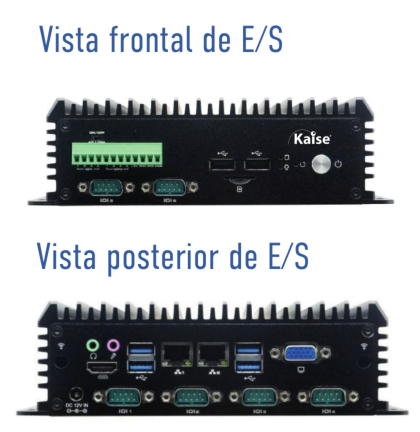
\includegraphics[width=.75\textwidth]{graficos/kaise}
    \end{minipage}
    \hfill
    \begin{minipage}[b]{0.48\textwidth}
        \begin{itemize}
            \item \textbf{Tipo:} PC industrial fanless compacta.
            \item \textbf{Procesador:} Intel Celeron J6412.
            \item \textbf{Memoria instalada:} 8~GB DDR4.
            \item \textbf{Red:} 2 interfaces Gigabit Ethernet.
            \item \textbf{Puertos E/S:} 6 puertos RS232 (2 RS485), \\2 USB 2.0, 4 USB 3.0, 8 GPIO. 
            \item \textbf{Alimentaci�n:} entrada DC de 12~V.
            \vspace{10px}
        \end{itemize}
    \end{minipage}
    \caption{Computadora principal embarcada para el control del sistema instrumental de la boya EAMMRA.}
    \label{fig:kaise}
\end{figure}

La disponibilidad de m�ltiples interfaces serie resulta especialmente relevante para la integraci�n simult�nea de perif�ricos industriales, meteorol�gicos, energ�ticos y satelitales. Asimismo, el dise�o sin ventilador reduce partes m�viles y mejora la aptitud del equipo para operaci�n embarcada.

\vspace{10px}
\noindent \textbf{Sensor ambiental AHT10.}

El AHT10 es un sensor digital de temperatura y humedad relativa. En el sistema EAMMRA se utiliza para adquirir variables ambientales internas o de entorno inmediato, con bajo consumo y bajo ancho de banda. Estas mediciones permiten caracterizar condiciones de operaci�n y aportar informaci�n de diagn�stico sobre el ambiente donde se encuentra alojada la electr�nica.

    \begin{minipage}[c]{0.68\textwidth}
        \begin{itemize}
		    \item \textbf{Variables medidas:} temperatura y humedad relativa.
		    \item \textbf{Interfaz el�ctrica:} bus I2C.
		    \item \textbf{Direcci�n I2C de referencia:} \texttt{0x38}.
		    \item \textbf{Rango t�pico de humedad relativa:} 0 a 100~\%RH.
		    \item \textbf{Rango t�pico de temperatura:} \(-40~^{\circ}\mathrm{C}\) a \(85~^{\circ}\mathrm{C}\).
		    \item \textbf{Biblioteca de acceso:} \texttt{smbus2}.
   		    \item \textbf{Uso en la boya:} diagn�stico de condiciones internas.
	    \end{itemize}
    \end{minipage}
    \hfill
    \begin{minipage}[c]{0.3\textwidth}
        \begin{figure}[htbp]
        \centering
        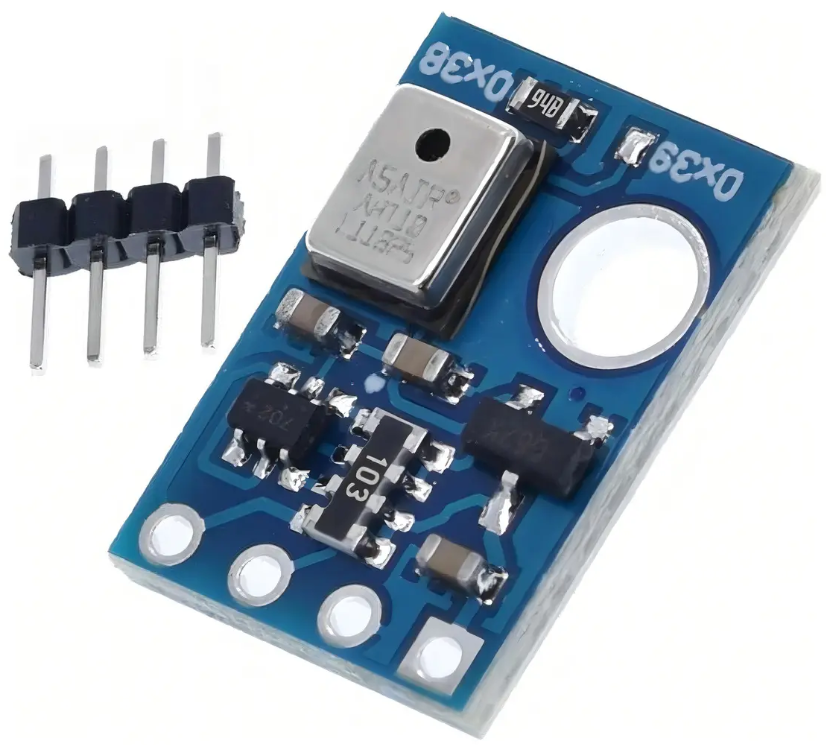
\includegraphics[width=.2\textwidth]{graficos/aht10.png}
        \caption{Computadora principal embarcada para el control del sistema instrumental de la boya EAMMRA.}
	    \label{fig:aht10}
	    \end{figure}
    \end{minipage}

    
\pagebreak

\begin{itemize}
    \item \textbf{Variables medidas:} temperatura y humedad relativa.
    \item \textbf{Interfaz el�ctrica:} bus I2C.
    \item \textbf{Direcci�n I2C de referencia:} \texttt{0x38}.
    \item \textbf{Rango t�pico de humedad relativa:} 0 a 100~\%RH.
    \item \textbf{Rango t�pico de temperatura:} aproximadamente \(-40~^{\circ}\mathrm{C}\) a \(85~^{\circ}\mathrm{C}\), seg�n hoja de datos.
    \item \textbf{Uso en la boya:} monitoreo ambiental y diagn�stico de condiciones internas.
    \item \textbf{Biblioteca de acceso:} \texttt{smbus2}.
\end{itemize}

El protocolo de comunicaci�n se basa en comandos I2C de inicializaci�n, disparo de medici�n y lectura de respuesta. .

%En la implementaci�n del sistema, el m�dulo de bajo nivel realiza la apertura del bus, verifica la presencia del dispositivo, ejecuta mediciones y valida que los valores obtenidos se encuentren dentro de rangos f�sicamente plausibles.

\vspace{10px}
\noindent \textbf{Unidad inercial MPU6050.}

El MPU6050 es una unidad inercial de seis grados de libertad que integra aceler�metro triaxial y gir�scopo triaxial. En EAMMRA se utiliza para registrar variables asociadas al movimiento de la boya, las cuales pueden aportar informaci�n para diagn�stico mec�nico, identificaci�n de eventos din�micos y posterior correlaci�n con registros ac�sticos.

\begin{itemize}
    \item \textbf{Variables medidas:} aceleraci�n triaxial, velocidad angular triaxial.
    \item \textbf{Interfaz el�ctrica:} bus I2C.
    \item \textbf{Direcciones I2C posibles:} \texttt{0x68} y \texttt{0x69}.
    \item \textbf{Rangos configurables de aceler�metro:} \(\pm 2g\), \(\pm 4g\), \(\pm 8g\), \(\pm 16g\).
    \item \textbf{Rangos configurables de gir�scopo:} \(\pm 250\), \(\pm 500\), \(\pm 1000\), \(\pm 2000~^{\circ}/\mathrm{s}\).
    \item \textbf{Velocidad de bus:} compatible con I2C de hasta 400~kHz.
    \item \textbf{Uso en la boya:} registro de movimiento y correlaci�n con eventos mec�nicos.
\end{itemize}

El m�dulo de bajo nivel configura los registros internos del sensor, verifica el identificador del dispositivo y convierte las lecturas crudas a unidades f�sicas. La existencia de rangos programables permite adaptar la sensibilidad del sensor a escenarios de operaci�n con diferente nivel de movimiento.

\vspace{10px}
\noindent \textbf{Receptor AIS/GPS.}

El subsistema AIS/GPS provee informaci�n de posicionamiento, fecha, hora y datos de navegaci�n. En la implementaci�n actual se comunica con la computadora principal mediante puerto serie y entrega sentencias compatibles con el formato NMEA. La informaci�n de posici�n y tiempo es esencial para asociar las mediciones ac�sticas, meteorol�gicas y ambientales con una ubicaci�n y una referencia temporal.

\begin{itemize}
    \item \textbf{Variables principales:} latitud, longitud, fecha, hora, calidad de fix, n�mero de sat�lites y diluci�n horizontal de precisi�n.
    \item \textbf{Interfaz el�ctrica:} puerto serie.
    \item \textbf{Formato de datos:} sentencias NMEA.
    \item \textbf{Sentencias GPS de inter�s:} RMC, GGA, GLL, GSA, GSV y TXT, seg�n disponibilidad.
    \item \textbf{Uso en la boya:} georreferenciaci�n, sincronizaci�n temporal y soporte a seguridad mar�tima.
\end{itemize}

El m�dulo de software valida el checksum de las sentencias NMEA, convierte coordenadas desde el formato grados-minutos a grados decimales y mantiene un estado de navegaci�n actualizado.

\vspace{10px}
\noindent \textbf{Anem�metro ultras�nico WindSonic.}

El WindSonic es un anem�metro ultras�nico de dos ejes utilizado para medir velocidad y direcci�n del viento. Al no poseer partes m�viles, resulta adecuado para operaci�n prolongada en ambiente mar�timo, donde los anem�metros mec�nicos pueden degradarse por desgaste, salinidad o incrustaciones. La medici�n de viento es importante porque las condiciones de superficie influyen directamente sobre el ruido ambiente submarino.

\begin{itemize}
    \item \textbf{Variables medidas:} velocidad y direcci�n del viento.
    \item \textbf{Principio de medici�n:} ultrasonido, sin partes m�viles.
    \item \textbf{Rango t�pico de velocidad:} hasta 60~m/s, seg�n variante.
    \item \textbf{Rango de direcci�n:} 0 a 360 grados.
    \item \textbf{Interfaz el�ctrica:} puerto serie.
    \item \textbf{Protocolos disponibles seg�n versi�n:} RS232, RS422, RS485 y salida NMEA.
    \item \textbf{Configuraci�n serie de referencia:} 8 bits de datos, sin paridad, 1 bit de parada.
    \item \textbf{Uso en la boya:} caracterizaci�n meteorol�gica y correlaci�n con ruido ambiente submarino.
\end{itemize}

El m�dulo de bajo nivel implementa la consulta al instrumento, la verificaci�n de respuesta, el an�lisis de datos recibidos y la acumulaci�n de muestras. La identificaci�n del dispositivo se realiza mediante comandos de consulta sobre la interfaz serie, de acuerdo con el protocolo configurado para el equipo.

\textbf{Controlador solar MPPT XTRA2210.}

El XTRA2210 es un controlador de carga solar de tipo MPPT. Su funci�n es administrar la transferencia de energ�a entre los paneles solares y el banco de bater�as, con el objetivo de maximizar la potencia extra�da del arreglo fotovoltaico y proteger la bater�a durante los ciclos de carga y descarga. En EAMMRA constituye el perif�rico principal de supervisi�n energ�tica.

\begin{itemize}
    \item \textbf{Modelo:} XTRA2210N, familia XTRA-N.
    \item \textbf{Tipo:} controlador de carga solar MPPT.
    \item \textbf{Corriente nominal de carga:} 20~A.
    \item \textbf{Tensi�n nominal del sistema:} 12/24~V, con detecci�n autom�tica seg�n configuraci�n del controlador.
    \item \textbf{Interfaz de comunicaci�n:} RS485.
    \item \textbf{Protocolo:} Modbus.
    \item \textbf{Uso en la boya:} supervisi�n de energ�a, diagn�stico del sistema fotovoltaico y seguimiento del estado de bater�a.
\end{itemize}

El m�dulo de software consulta registros asociados a entrada fotovoltaica, bater�a, carga, temperaturas y estado de carga. Entre las variables de inter�s se incluyen tensi�n y corriente de panel, tensi�n y corriente de bater�a, potencia de carga, temperatura de bater�a, temperatura interna del dispositivo y estado de carga estimado. Estos datos permiten evaluar la disponibilidad energ�tica de la boya y aportan informaci�n para diagn�stico operativo.

\textbf{Subsistema ac�stico.}

El subsistema ac�stico constituye la cadena de adquisici�n principal de la boya EAMMRA. Est� compuesto por hidr�fonos piezoel�ctricos calibrados, preamplificadores DAS-1 y DAS-2, y una placa de audio USB Behringer UMC202HD. Su funci�n es adquirir se�ales de presi�n ac�stica subacu�tica, convertirlas a archivos de audio digital y habilitar el procesamiento posterior.

\begin{itemize}
    \item \textbf{Sensores primarios:} hidr�fonos piezoel�ctricos calibrados.
    \item \textbf{Acondicionamiento anal�gico:} preamplificadores DAS-1 y DAS-2.
    \item \textbf{Placa de adquisici�n:} Behringer UMC202HD.
    \item \textbf{Interfaz con computadora principal:} USB audio.
    \item \textbf{Cantidad de canales de adquisici�n:} 2 canales simult�neos.
    \item \textbf{Frecuencia de muestreo:} hasta 192~kHz por canal.
    \item \textbf{Resoluci�n nominal de la placa:} 24~bits.
    \item \textbf{Formato de archivo generado:} WAV.
    \item \textbf{Uso en la boya:} adquisici�n de se�ales ac�sticas submarinas y generaci�n de archivos para procesamiento local.
\end{itemize}

Los preamplificadores DAS-1 y DAS-2 fueron dise�ados para adaptar la se�al de los hidr�fonos a la placa de adquisici�n, con bajo ruido propio, respuesta extendida hasta 100~kHz y corte en bajas frecuencias. El dise�o de la etapa de preamplificaci�n responde a la necesidad de elevar se�ales de baja amplitud sin degradar la detectabilidad de eventos ac�sticos de inter�s \cite{AS0518_Preamp}. La caracterizaci�n del conjunto placa-preamplificador se documenta en la Nota T�cnica AS~02/26, donde se relevaron la respuesta en frecuencia, la figura de ruido propio y el crosstalk entre canales \cite{Cinquini2026_AS0226}.

En el software, el m�dulo de bajo nivel asociado a la placa de audio detecta dispositivos compatibles, valida cantidad de canales, frecuencia de muestreo y formato de audio, administra la adquisici�n y escribe los archivos WAV en el directorio de grabaciones. Tambi�n aplica verificaciones de disponibilidad de almacenamiento antes de iniciar una adquisici�n, con el objetivo de evitar grabaciones incompletas o p�rdida de datos previos.

\textbf{M�dem satelital Iridium SBD.}

El subsistema Iridium permite la transmisi�n remota de mensajes mediante el servicio SBD. En la boya se utiliza para enviar informaci�n compacta de estado, diagn�stico y resultados seleccionados del procesamiento ac�stico. La telemetr�a satelital no reemplaza al almacenamiento local, sino que provee un canal de supervisi�n remota y recuperaci�n parcial de informaci�n cr�tica.

\begin{itemize}
    \item \textbf{Tecnolog�a:} Iridium SBD.
    \item \textbf{Interfaz el�ctrica:} RS232.
    \item \textbf{Protocolo de control:} comandos AT.
    \item \textbf{Configuraci�n serie de referencia:} 8 bits de datos, sin paridad, 1 bit de parada.
    \item \textbf{Tipo de mensajes:} mensajes binarios de estado y resultados compactos de procesamiento.
    \item \textbf{Uso en la boya:} diagn�stico remoto, supervisi�n de continuidad operativa y transmisi�n de informaci�n resumida.
\end{itemize}

El servicio SBD impone restricciones de tama�o de mensaje, por lo que los datos transmitidos deben seleccionarse, compactarse y codificarse de manera eficiente. En la arquitectura del sistema, la transmisi�n se ejecuta en ciclos regulares definidos por el planificador de tareas y se desacopla de la finalizaci�n inmediata de una adquisici�n. Esta estrategia evita dependencias temporales r�gidas entre adquisici�n, procesamiento y comunicaci�n satelital.

\textbf{Almacenamiento local.}

El almacenamiento local constituye el repositorio primario de datos de la boya. All� se conservan archivos WAV de audio, mediciones estructuradas, resultados de procesamiento, registros de eventos, logs de ejecuci�n y estados del sistema. La telemetr�a satelital transmite s�lo un subconjunto resumido de esta informaci�n.

\begin{itemize}
    \item \textbf{Datos almacenados:} archivos WAV, mediciones JSONL, resultados JSON, logs y estados de sistema.
    \item \textbf{Funci�n principal:} preservaci�n de datos completos de campa�a.
    \item \textbf{Funci�n secundaria:} soporte a diagn�stico posterior y trazabilidad operativa.
    \item \textbf{Criterio de dise�o:} priorizar la integridad de datos ya adquiridos frente a nuevas adquisiciones.
\end{itemize}

La pol�tica de almacenamiento asociada a la adquisici�n ac�stica es conservadora. Antes de iniciar una grabaci�n se verifica la existencia del directorio de destino, la disponibilidad de espacio libre y el tama�o m�ximo esperado del archivo WAV. Si las condiciones no son aceptables, el sistema rechaza la adquisici�n y registra la causa. Esta decisi�n protege la informaci�n previamente adquirida y reduce el riesgo de archivos incompletos durante operaci�n aut�noma.

\subsection{Entorno de Software, Lenguaje y Dependencias}\label{subsec:entorno_de_software_lenguaje_y_dependencias}

El lenguaje principal utilizado para el desarrollo del sistema embebido de control fue Python~3. La elecci�n de este lenguaje responde a la necesidad de integrar, en una misma plataforma de software, acceso a perif�ricos, comunicaci�n serie, adquisici�n de audio, procesamiento de se�ales, almacenamiento estructurado, telemetr�a, pruebas automatizadas y herramientas de simulaci�n. Python ofrece una sintaxis expresiva, amplia disponibilidad de bibliotecas y buena integraci�n con sistemas GNU/Linux, caracter�sticas adecuadas para una computadora principal embarcada.

En este proyecto, Python se utiliza como lenguaje de coordinaci�n del sistema. Las funciones de lectura de perif�ricos, procesamiento, persistencia, transmisi�n y control de estado se organizan mediante m�dulos independientes, M�quinas de Estados Finitos, un enrutador de eventos y un planificador de tareas central. De esta manera, el lenguaje no se emplea s�lo para scripts auxiliares, sino como base de la aplicaci�n principal de control de la boya.

Para aislar las dependencias del proyecto respecto del sistema operativo base se utiliz� un entorno virtual de Python, ubicado convencionalmente en el directorio \texttt{.venv}. Este mecanismo permite mantener un int�rprete y un conjunto de bibliotecas espec�ficos para la aplicaci�n, lo que reduce interferencias con otros paquetes instalados en el sistema y favorece la reproducibilidad del entorno de ejecuci�n \cite{PythonVenvDocs,PyPAPackagingGuide}.

La instalaci�n del entorno se realiza desde la ra�z del repositorio. En primer lugar, se requiere disponer de ciertas dependencias del sistema operativo asociadas al acceso a hardware, interfaces de bajo nivel y adquisici�n de audio. En particular, el proyecto recomienda instalar los paquetes:

\begin{verbatim}
sudo apt-get update
sudo apt-get install -y portaudio19-dev python3-dev i2c-tools
\end{verbatim}

Luego, el entorno virtual se activa mediante:

\begin{verbatim}
source .venv/bin/activate
\end{verbatim}

y las dependencias de Python se instalan mediante \texttt{pip}. Para una instalaci�n orientada exclusivamente a ejecuci�n, sin herramientas de prueba, se utiliza:

\begin{verbatim}
python -m pip install -r support/requirements.txt
\end{verbatim}

Para desarrollo, verificaci�n y ejecuci�n de pruebas automatizadas, se instala el conjunto ampliado de dependencias:

\begin{verbatim}
python -m pip install -r support/requirements-dev.txt
\end{verbatim}

El archivo \texttt{support/requirements.txt} define las bibliotecas necesarias para la operaci�n nominal del sistema. Las versiones se especifican mediante restricciones de compatibilidad, salvo en el caso de \texttt{PyAudio}, cuya versi�n se fija expl�citamente.

\begin{table}[htbp]
    \centering
    \caption{Dependencias principales de ejecuci�n del sistema.}
    \label{tab:runtime-dependencies}
    \begin{tabular}{lll}
        \hline
        \textbf{Biblioteca} & \textbf{Versi�n requerida} & \textbf{Uso principal} \\
        \hline
        \texttt{numpy}    & \texttt{>=2.0,<3}    & C�lculo num�rico y procesamiento de datos. \\
        \texttt{pandas}   & \texttt{>=2.0,<4}    & Manejo de datos tabulares y archivos estructurados. \\
        \texttt{scipy}    & \texttt{>=1.14,<2}   & Procesamiento cient�fico y an�lisis de se�ales. \\
        \texttt{PyAudio}  & \texttt{==0.2.14}    & Interfaz con PortAudio para adquisici�n de audio. \\
        \texttt{pyserial} & \texttt{>=3.5,<4}    & Comunicaci�n con perif�ricos mediante puertos serie. \\
        \texttt{smbus2}   & \texttt{>=0.5,<1}    & Comunicaci�n con dispositivos sobre bus I2C. \\
        \hline
    \end{tabular}
\end{table}

El archivo \texttt{support/requirements-dev.txt} extiende las dependencias de ejecuci�n e incorpora herramientas espec�ficas para desarrollo, pruebas y generaci�n de gr�ficos.

\begin{table}[htbp]
    \centering
    \caption{Dependencias adicionales de desarrollo y pruebas.}
    \label{tab:dev-dependencies}
    \begin{tabular}{lll}
        \hline
        \textbf{Biblioteca} & \textbf{Versi�n requerida} & \textbf{Uso principal} \\
        \hline
        \texttt{pytest}     & \texttt{>=8,<10}     & Ejecuci�n de pruebas automatizadas. \\
        \texttt{pytest-cov} & \texttt{>=7,<8}      & Medici�n de cobertura de pruebas. \\
        \texttt{matplotlib} & \texttt{>=3.8,<4}    & Generaci�n de gr�ficos y reportes t�cnicos. \\
        \hline
    \end{tabular}
\end{table}

Esta separaci�n entre dependencias de ejecuci�n y dependencias de desarrollo permite distinguir el entorno m�nimo requerido para operar la boya del entorno ampliado utilizado durante integraci�n, depuraci�n y validaci�n. En una plataforma embebida operativa resulta conveniente mantener el entorno de ejecuci�n tan acotado como sea posible, mientras que en laboratorio se justifica incorporar herramientas adicionales para pruebas, an�lisis y generaci�n de evidencia.

El uso del entorno virtual tambi�n facilita la ejecuci�n expl�cita de comandos desde el int�rprete asociado al proyecto. Por ejemplo, la aplicaci�n principal puede iniciarse con:

\begin{verbatim}
PYTHONPATH=. .venv/bin/python main.py
\end{verbatim}

mientras que la suite de pruebas sin hardware puede ejecutarse mediante:

\begin{verbatim}
PYTHONPATH=. .venv/bin/python -m pytest -m "not hardware" -q
\end{verbatim}

De esta manera, el entorno de trabajo queda definido por tres niveles complementarios: paquetes del sistema operativo necesarios para interfaces f�sicas, entorno virtual Python para aislamiento de bibliotecas y archivos \texttt{requirements} para reproducir las versiones compatibles de las dependencias del proyecto. Esta organizaci�n contribuye a la trazabilidad, repetibilidad y mantenibilidad del software embarcado.

\subsection{Herramientas de Desarrollo y Calidad de C�digo}\label{subsec:herramientas_de_desarrollo_y_calidad_de_codigo}

El desarrollo del software se gestion� mediante un repositorio Git alojado en GitHub. El repositorio integra en una �nica base de trabajo el c�digo fuente del sistema embebido, los archivos de configuraci�n, los manuales de perif�ricos, los scripts auxiliares, los datos de soporte y los ensayos automatizados \cite{BoyaRepo}. En esta secci�n se describe el repositorio como herramienta de desarrollo, control de versiones y trazabilidad. La organizaci�n concreta del c�digo fuente se detalla en la Secci�n~\ref{sec:diseno_e_implementacion}.

Para asistir el desarrollo se utiliz� Visual Studio Code con la extensi�n Pylance. Esta extensi�n provee soporte de lenguaje para Python, con funciones de autocompletado, navegaci�n de s�mbolos, an�lisis de tipos, detecci�n temprana de errores y asistencia durante la edici�n del c�digo. Su uso resulta especialmente �til en un proyecto modular, donde las interfaces entre m�dulos, clases, funciones y estructuras de datos deben mantenerse consistentes a lo largo del desarrollo \cite{PylanceDocs}.

Asimismo, se prev� incorporar Pylint como herramienta de an�lisis est�tico. Pylint permite inspeccionar el c�digo fuente sin ejecutarlo, detectar errores probables, identificar problemas de estilo, advertir sobre construcciones potencialmente confusas y sugerir refactorizaciones. En un sistema embebido aut�nomo, este tipo de herramienta contribuye a reducir defectos antes de la etapa de integraci�n con hardware, mejorar la mantenibilidad del c�digo y reforzar criterios homog�neos de calidad \cite{PylintDocs}.

Tambi�n se incorpora Black como formateador autom�tico de c�digo. Su funci�n es aplicar un estilo de formato consistente y reproducible sobre los archivos Python. Esta decisi�n reduce diferencias manuales de formato entre desarrolladores, facilita las revisiones de c�digo, simplifica la interpretaci�n de cambios entre versiones y favorece una base de c�digo visualmente homog�nea \cite{BlackDocs}.

Para la ejecuci�n de pruebas automatizadas se utiliz� \texttt{pytest}, un framework de pruebas para Python orientado a la escritura de tests unitarios, funcionales y de integraci�n con una sintaxis simple y legible \cite{pytestDocs}. A diferencia de enfoques m�s verbosos, \texttt{pytest} permite expresar verificaciones mediante sentencias \texttt{assert} convencionales, descubrir autom�ticamente archivos y funciones de prueba siguiendo convenciones de nombre, definir contextos reutilizables mediante \emph{fixtures} y organizar subconjuntos de ensayos mediante marcas o configuraciones espec�ficas.

En el presente desarrollo, \texttt{pytest} se emple� como herramienta principal para verificar el comportamiento de m�dulos individuales, validar la l�gica de las M�quinas de Estados Finitos, ejecutar pruebas con componentes simulados y separar ensayos que no requieren hardware de aquellos destinados a perif�ricos reales. Su incorporaci�n permite mejorar la repetibilidad de los ensayos, reducir regresiones durante el desarrollo y sostener una estrategia de verificaci�n compatible con una arquitectura modular y mantenible.

En conjunto, el entorno de desarrollo se estructura en tres niveles complementarios: el int�rprete Python y su entorno virtual para aislar dependencias; las bibliotecas de ejecuci�n y desarrollo declaradas en los archivos de requerimientos; y las herramientas de asistencia, an�lisis est�tico, formateo y prueba empleadas para mejorar la calidad del c�digo. Esta combinaci�n permite sostener un flujo de desarrollo controlado, repetible y auditable, compatible con la documentaci�n t�cnica y la validaci�n progresiva del sistema.

\subsection{Arquitectura Funcional General del Sistema}\label{subsec:arquitectura_funcional_general_del_sistema}

La arquitectura general del sistema se basa en una organizaci�n modular orientada a eventos. Cada subsistema se representa mediante una M�quina de Estados Finitos que encapsula sus estados, transiciones, acciones y condiciones de error. La comunicaci�n entre m�dulos se realiza mediante mensajes, y un enrutador de eventos act�a como intermediario encargado de distribuir informaci�n entre productores y consumidores.

Desde un punto de vista funcional, la arquitectura puede representarse mediante las siguientes capas:

\begin{itemize}
    \item \textbf{Capa de hardware:} comprende sensores, placa de audio, m�dem satelital, controlador solar, interfaces serie, buses I2C, almacenamiento y dispositivos f�sicos asociados.
    \item \textbf{Capa de bajo nivel:} implementa el acceso directo a cada dispositivo o servicio espec�fico. Incluye inicializaci�n de interfaces, lectura de sensores, adquisici�n de audio, comunicaci�n AT/SBD, lectura de controladores de energ�a y funciones auxiliares de hardware.
    \item \textbf{Capa de control por estados:} implementa la l�gica de estado de cada m�dulo. Cada M�quina de Estados Finitos recibe eventos, ejecuta acciones, valida resultados, registra estados y comunica eventos de salida al resto del sistema.
    \item \textbf{Capa de enrutamiento:} centraliza la distribuci�n de mensajes y evita dependencias directas entre m�dulos.
    \item \textbf{Capa de planificaci�n:} ejecuta el planificador de tareas central, responsable de disparar adquisiciones peri�dicas, transmisiones, tareas de mantenimiento y ciclos operativos de acuerdo con la configuraci�n vigente.
    \item \textbf{Capa de persistencia:} administra la escritura de mediciones, logs, estados, archivos de audio, resultados procesados y mensajes preparados para transmisi�n.
    \item \textbf{Capa de telemetr�a:} prepara y transmite mensajes binarios mediante Iridium SBD, incluidos estados de sistema y resultados seleccionados de procesamiento ac�stico.
\end{itemize}

El flujo general de operaci�n comienza con la inicializaci�n de configuraciones, m�dulos y recursos del sistema. Una vez iniciado el proceso principal, el planificador de tareas central dispara eventos de adquisici�n de acuerdo con intervalos definidos. Los sensores ambientales, meteorol�gicos, inerciales, de posici�n y energ�a generan registros peri�dicos. Para los ensayos de verificaci�n, la adquisici�n ac�stica se ejecuta con una periodicidad menor que la de los sensores de bajo ancho de banda, debido al mayor volumen de datos generado.

El m�dulo de adquisici�n ac�stica realiza la grabaci�n de audio y genera archivos WAV con metadatos asociados. Al finalizar una adquisici�n v�lida, el resultado queda disponible para el m�dulo de procesamiento de audio, que procesa el archivo y genera resultados compactos, persistidos en formato estructurado. Estos resultados pueden ser posteriormente seleccionados por el subsistema Iridium para su transmisi�n satelital.

La telemetr�a Iridium se organiza en ciclos regulares. El sistema puede transmitir mensajes de estado que resumen la condici�n operativa de las M�quinas de Estados Finitos, los m�dulos de bajo nivel, la disponibilidad de almacenamiento, el estado energ�tico y el tiempo desde el arranque. Tambi�n puede transmitir resultados derivados del procesamiento de audio, compactados en formato binario para adecuarse a las restricciones de tama�o del enlace SBD.

El dise�o evita que la transmisi�n satelital dependa directamente de la finalizaci�n de una adquisici�n. En su lugar, el sistema registra la disponibilidad del �ltimo resultado v�lido y el planificador de tareas gobierna los momentos de transmisi�n. Esta decisi�n reduce acoplamientos, simplifica el control temporal del enlace satelital y permite mantener un comportamiento predecible aun cuando alguna tarea se demore, falle o produzca datos incompletos.

\subsection{Requerimientos Funcionales y No Funcionales}\label{subsec:requerimientos_funcionales_y_no_funcionales}

Los requerimientos funcionales del sistema surgen de la necesidad de controlar una boya instrumental aut�noma con m�ltiples subsistemas integrados. En t�rminos generales, el sistema debe ser capaz de adquirir datos, validarlos, almacenarlos, procesarlos parcialmente y transmitir informaci�n seleccionada en forma remota.

Los requerimientos funcionales principales son:

\begin{itemize}
    \item Adquirir mediciones ambientales de temperatura y humedad.
    \item Adquirir mediciones inerciales de aceleraci�n y velocidad angular.
    \item Adquirir informaci�n de posicionamiento, tiempo y datos de navegaci�n mediante AIS/GPS.
    \item Adquirir mediciones meteorol�gicas de velocidad y direcci�n del viento.
    \item Relevar variables el�ctricas del sistema de alimentaci�n, incluidos par�metros asociados a panel solar, carga y bater�a.
    \item Ejecutar adquisiciones ac�sticas mediante placa de audio USB y almacenar archivos WAV con metadatos asociados.
    \item Procesar archivos de audio para obtener productos compactos compatibles con almacenamiento local y telemetr�a satelital.
    \item Registrar mediciones en archivos persistentes con formato estructurado y unidades expl�citas.
    \item Registrar logs de ejecuci�n, eventos relevantes, errores, advertencias y condiciones de diagn�stico.
    \item Transmitir mensajes de estado de sistema mediante Iridium SBD.
    \item Transmitir resultados seleccionados de procesamiento ac�stico mediante Iridium SBD.
    \item Ejecutar tareas peri�dicas mediante un planificador de tareas central configurable.
    \item Representar el comportamiento de cada m�dulo mediante M�quinas de Estados Finitos.
    \item Permitir ejecuci�n con hardware real, con todos los m�dulos simulados o con simulaci�n parcial de m�dulos seleccionados.
    \item Permitir pruebas automatizadas sin hardware y pruebas espec�ficas contra hardware real.
    \item Mantener archivos de configuraci�n editables para adaptar intervalos, rutas, par�metros de adquisici�n, habilitaci�n de telemetr�a y uso de \emph{mocks}.
\end{itemize}

Los requerimientos no funcionales responden a las restricciones propias de una plataforma aut�noma embarcada. Entre ellos se destacan:

\begin{itemize}
    \item \textbf{Autonom�a operativa:} el sistema debe ejecutar ciclos de adquisici�n, almacenamiento y transmisi�n sin intervenci�n humana continua.
    \item \textbf{Robustez:} el sistema debe tolerar fallas parciales de m�dulos, errores de lectura, indisponibilidad transitoria de perif�ricos y condiciones de comunicaci�n no ideales.
    \item \textbf{Persistencia segura:} los datos adquiridos no deben perderse por fallas evitables de software, configuraciones ambiguas o pol�ticas agresivas de liberaci�n de espacio.
    \item \textbf{Bajo consumo relativo:} el software debe permitir ciclos de adquisici�n y transmisi�n compatibles con el presupuesto energ�tico disponible.
    \item \textbf{Mantenibilidad:} la separaci�n entre bajo nivel, M�quinas de Estados Finitos, enrutador de eventos y planificador de tareas debe facilitar la modificaci�n de m�dulos individuales sin afectar la arquitectura completa.
    \item \textbf{Extensibilidad:} la arquitectura debe permitir la incorporaci�n futura de nuevos sensores, nuevos productos de procesamiento o nuevos formatos de telemetr�a.
    \item \textbf{Verificabilidad:} el comportamiento del sistema debe poder probarse mediante tests automatizados, ejecuci�n con \emph{mocks}, ensayos de bajo nivel y pruebas de integraci�n.
    \item \textbf{Trazabilidad:} las mediciones, eventos, configuraciones y resultados de prueba deben poder relacionarse con m�dulos, horarios de ejecuci�n y condiciones operativas.
    \item \textbf{Degradaci�n controlada:} ante una falla, el sistema debe registrar la condici�n, conservar datos previos, evitar acciones inseguras y continuar operando en la medida de lo posible.
    \item \textbf{Diagn�stico remoto:} los mensajes satelitales deben permitir inferir el estado general de la boya, incluida la salud de m�dulos, almacenamiento, energ�a y continuidad operativa.
\end{itemize}

En conjunto, estos requerimientos justifican la arquitectura adoptada. La combinaci�n de m�dulos de bajo nivel, M�quinas de Estados Finitos, enrutador de eventos, planificador de tareas central, almacenamiento estructurado, telemetr�a binaria, pruebas automatizadas y soporte de simulaci�n permite abordar la complejidad de una boya operativa sin concentrar toda la l�gica en un bloque monol�tico. La Introducci�n Espec�fica presentada en esta secci�n establece, por lo tanto, el marco t�cnico necesario para comprender las decisiones de dise�o e implementaci�n desarrolladas en las secciones siguientes.


\section{Dise�o e Implementaci�n}
\label{sec:diseno_e_implementacion}
\subsection{Arquitectura del sistema}
\subsection{Proceso principal y enrutamiento de eventos}
\subsection{Planificador y gesti�n de tareas}
\subsection{M�dulos de sensores}
\subsubsection{Sensores ambientales (AHT10, MPU6050)}
\subsubsection{Sensores meteorol�gicos y de posici�n}
\subsubsection{Procesamiento de audio}
\subsubsection{Gesti�n de energ�a}
\subsection{Telemetr�a satelital (Iridium SBD)}
\subsection{Protocolos y formatos de datos}
\subsection{Almacenamiento y pol�ticas de persistencia}

\section{Pruebas y Ensayos}
\subsection{Pruebas unitarias y de integraci�n}
\subsection{Tests de bajo nivel y simulaciones (mocks)}
\subsection{Ensayos operacionales en laboratorio}
\subsection{Pruebas de campo y telemetr�a}
\subsection{Resultados obtenidos}

\section{Conclusiones y Trabajo Futuro}
\subsection{Conclusiones}
\subsection{Logros alcanzados}
\subsection{Dificultades encontradas y lecciones aprendidas}
\subsection{Trabajo futuro}
\subsubsection{Mejoras propuestas}
\subsubsection{Nuevas funcionalidades}
\subsubsection{Escalabilidad y mantenimiento del sistema}


% =====================================================================================================
% =====================================================================================================
% P�GINA DE REFERENCIAS
% =====================================================================================================
% =====================================================================================================

\clearpage
\vspace{4pc}
\addcontentsline{toc}{section}{REFERENCIAS}
\bibliographystyle{apa-good}	% (uses file "plain.bst")
\bibliography{7_Referencias}	% Ac� est� la base de datos de referencias. Espera el archivo "7_Referencias.bib"

\clearpage

% =====================================================================================================
% =====================================================================================================
% AP�NDICE
% =====================================================================================================
% =====================================================================================================


% Reseteo y cambio de numeraci�n para los ap�ndices
\setcounter{section}{0}
\renewcommand\appendix{\Roman{section}}
%\def\thesection{\Roman{section}}

%% =================================================================================================
% =================================================================================================
%\appendix
% =================================================================================================
% =================================================================================================
\appendix
\appendixpage
\addappheadtotoc
\section{\textit{Scripts} computacionales.}


\section{Circuitos de electr�nica adicional (borneras).}

\section{Especificaciones de partes constitutivas.}

\section{Planos.}





\end{document}
